\subsection{Pengujian Gerakan Linier dan Estimasi Posisi di Simulasi}
\label{subsec:liniersimulasi}

\begin{figure}[ht]
  \centering
  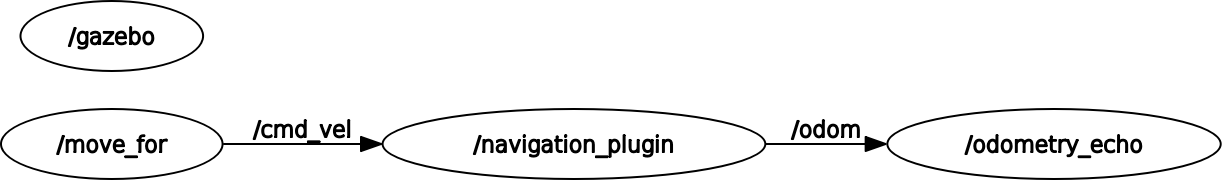
\includegraphics[scale=0.3]{gambar/rosgraph-navigation-plugin.png}
  \caption{Relasi antar-\emph{node} dari pengujian gerakan linier dan estimasi posisi di simulasi.}
  \label{fig:rosgraphnavigationplugin}
\end{figure}

Pengujian gerakan linear dan estimasi posisi di simulasi dilakukan dengan cara menjalankan lingkungan \emph{outdoor} pada simulator Gazebo,
  menjalankan \emph{move for node} sebagai \emph{behavior node} dari pengujian,
  dan menjalankan \emph{odometry echo node} untuk menampilkan hasil estimasi posisi dari kalkulasi odometri robot.
Seperti yang terlihat pada gambar \ref{fig:rosgraphnavigationplugin},
  \emph{node} \lstinline{/move_for} akan mengirimkan \emph{topic} \lstinline{/cmd_vel} yang memerintahkan \emph{node} \lstinline{/navigation_plugin} untuk menggerakkan robot sesuai dengan data kecepatan yang ada di \emph{topic} tersebut,
  setelah itu \emph{node} \lstinline{/odometry_echo} akan menerima \emph{topic} \lstinline{/odom} yang menunjukkan estimasi posisi dari perhitungan yang dilakukan oleh \emph{node} \lstinline{/navigation_plugin}.

\begin{sidewaystable}
  \centering
  \caption{Hasil estimasi posisi dari gerakan linier pada robot di simulasi selama 3 detik.}
  \label{tb:gerakanliniersimulasi}
  \begin{tabular}{|c|c|c|c|c|c|c|c|c|c|c|}
    \hline \rowcolor[HTML]{E0E0E0}
    \multicolumn{2}{|c|}{Speed} &
    \multicolumn{3}{|c|}{Expected Pos} &
    \multicolumn{2}{|c|}{Measured Pos} &
    \multicolumn{4}{|c|}{Odometry Pos}
    \\ \hline \rowcolor[HTML]{E0E0E0}
    X (m/s) & Y (m/s) &
    X (m) & Y (m) & D (m) &
    X (m) & Y (m) &
    X (m) & Y (m) & E (m) & E (\%)
    \csvreader[head to column names]{data/gerakan_linier_simulasi.csv}{}{
      \\ \hline
      \speedx & \speedy &
      \expectedx & \expectedy & \expecteddistance &
      \measuredx & \measuredy &
      \odometryx & \odometryy & \odometryerror & \odometryerrorpercent
    }
    \\ \hline
  \end{tabular}
\end{sidewaystable}


Pengujian ini dilakukan dengan berbagai macam konfigurasi kecepatan X dan Y yang diperintahkan selama 10 detik.
Hasil pengujian ini bisa dilihat pada tabel \ref{tb:gerakanliniersimulasi}.
Pada tabel tersebut, nilai yang ada di kolom \emph{speed} adalah besar kecepatan yang diatur pada \emph{topic} \lstinline{/cmd_vel},
  nilai yang ada di kolom \emph{estimated position} didapatkan dari perkalian besar kecepatan dengan durasi pengujian,
  nilai yang ada di kolom \emph{measured position} didapatkan dari koordinat model yang ada di simulasi,
  dan terakhir nilai yang ada di kolom \emph{odometry position} didapatkan dari data yang ada pada \emph{topic} \lstinline{/odom}.

Dari data yang dihasilkan oleh pengujian ini dapat diketahui bahwa gerakan yang diperintahkan kepada robot cenderung menghasilkan posisi robot yang sesuai dengan posisi perkiraan (\emph{estimated position}).
Lebih lanjut, ketika hasil tersebut ditampilkan sebagai grafik,
  seperti yang terlihat pada gambar \ref{fig:grafikgerakanliniersimulasi},
  hasil yang didapatkan cenderung memiliki arah positif negatif yang sesuai dengan yang diharapkan (\emph{expected}) walaupun dengan \emph{error} jarak yang relatif tidak kecil (kurang lebih 1-2 meter).


\begin{figure}[ht]
  \centering
  \begin{tikzpicture}
    \begin{axis}[
        height=0.35\textwidth,
        width=0.9\textwidth,
        ylabel=X (meter),
        xticklabels={,,},
        ymajorgrids,
        bar width=3pt,
        ybar=0pt,
        xmin=0.1,
        xmax=12.9,
        xtick distance=1,
      ]
      \addplot table[x=index,y=expectedx,col sep=comma]{data/gerakan_linier_simulasi.csv};
      \addplot table[x=index,y=measuredx,col sep=comma]{data/gerakan_linier_simulasi.csv};
      \addplot table[x=index,y=odometryx,col sep=comma]{data/gerakan_linier_simulasi.csv};
    \end{axis}
  \end{tikzpicture}
  \begin{tikzpicture}
    \begin{axis}[
        height=0.35\textwidth,
        width=0.9\textwidth,
        ylabel=Y (meter),
        xlabel=Index,
        legend style={
          at={(0.5,-0.5)},
          anchor=north,
          legend columns=-1,
        },
        ymajorgrids,
        bar width=3pt,
        ybar=0pt,
        xmin=0.1,
        xmax=12.9,
        xtick distance=1,
      ]
      \addplot table[x=index,y=expectedy,col sep=comma]{data/gerakan_linier_simulasi.csv};
      \addplot table[x=index,y=measuredy,col sep=comma]{data/gerakan_linier_simulasi.csv};
      \addplot table[x=index,y=odometryy,col sep=comma]{data/gerakan_linier_simulasi.csv};
      \legend{Expected,Measured,Odometry}
    \end{axis}
  \end{tikzpicture}
  \caption{Grafik estimasi posisi dari gerakan linier pada robot di simulasi.}
  \label{fig:grafikgerakanliniersimulasi}
\end{figure}

